\chapter{Chromatin is globally compacted upon local damage, with nodes of repair in decondensed regions}

\paragraph*{} The advantage of FAI is in the fact that it could be useful for observing chromatin dynamics in live and fixed cells. Since we have introduced a 405nm laser in our widefield setup with the dual lamp housing (Fig. {\ref{fig:setup}}), we could microirradiate specific regions in hoechst-sensitized HeLa H2B-EGFP cells, and cause a localized damage, and monitor the change in the global state of chromatin compaction. Using DNA damage markers, we can follow damage repair dynamics along with chromatin compaction states. 

\section{Microirradiation induced damage}

\begin{figure}[!htp]
    {\hfill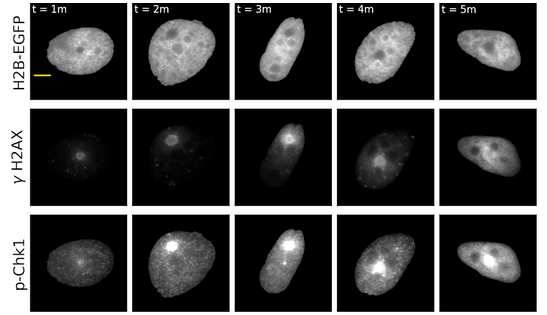
\includegraphics[clip,width=1\linewidth]{figures/pchk1.png}\hspace*{\fill}}
    \caption{Pan-nuclear induction of $\gamma$H2A.X in response to laser microirradiation. Hoechst-sensitized cells were microirradiated at intervals of 1 minute, with a different cell being irradiated every minute. Cells are fixed and stained for markers of damage response, $\gamma$H2A.X and phospho-Chk1 (a target of the ATR kinase). These are representative cells, but generally too induction of $\gamma$H2A.X is seen at the site of damage at the early timepoints, but it spreads out and there is pan-nuclear $\gamma$H2A.X induction 5-10 minutes onwards. Phospho-Chk1 is still enriched at the site of damage even at these later time-points. Scalebar is 5$\mu$m.}
    {\label{fig:chk1}}
\end{figure}


\paragraph*{} We used fluorescence anisotropy imaging to study the changes to chromatin structure that has undergone microirradiation induced DSBs as employed by previous studies \cite{kruhlak2006changes, BURGESS20141703,strickfaden2016poly}. We modified our FAI microscope to introduce a 405-nm laser into the light path and used Hoechst-sensitized cells to cause local double-strand breaks of the DNA. Minutes after irradiation, strong staining for $\gamma$H2AX and the phosphorylated form of Chk1 (p-Chk1, a target of the master DDR kinase ATR) was observed at the site of damage (Fig. {\ref{fig:chk1}}), which indicated that the damage response was in action. Using this microirradiation protocol, we collected anisotropy data for the damaged cells over a period of 2 h, imaged once every 5 min (Fig. {\ref{fig:live_an}}). Anisotropy at the site of the damage could not be ascertained due to localized photobleaching of H2B-EGFP upon irradiation, but the response of the rest of the chromatin, which did not see direct irradiation, could be followed. In comparison to the control undamaged cells (N = 13), the overall $\Delta$anisotropy value ($\Delta$anisotropy = rt – r0, where rt is the mean anisotropy at any given time point, and r0 is the mean anisotropy for the 0th time point) of the irradiated cells increased with time (Fig. {\ref{fig:timetrace}}), though the response was heterogeneous among cells ((Fig. {\ref{fig:hetero}})). And though the mean rise is small, one should keep in mind that anisotropy values are themselves fractional; also, mean anisotropy averages over regions where compaction increases and surrounding regions where it decreases correspondingly, keeping the changes in mean anisotropy small. This heterogeneity is captured in the anisotropy maps, and indeed a fraction of cells show formation of nodes of high local compaction even in regions that have not directly been damaged (Fig. {\ref{fig:live_an}}). To quantify this better and visualize the nodes, we thresholded the anisotropy map with a threshold value of “mean + 2 $\sigma$,” where mean is the mean anisotropy value of the nucleus before damage and $\sigma$ is the standard deviation of the mean. Values below the threshold are turned to gray, so that it becomes easier to visualize the high–anisotropy value pixels formed upon irradiation (Fig. {\ref{fig:thresholded}}). The formation of high-anisotropy nodes is reflected in the overall increase in high-anisotropy pixels for irradiated cells as compared with control cells. However, it should be noted that the control cells also show a fair degree of heterogeneity among themselves, and this could be because of toxic effects of the imaging excitation light, natural cell cycle–driven processes that causes chromatin compaction changes, or systematic changes to anisotropy with photobleaching. Nonetheless, the propensity for increased compaction in irradiated cells is clear and significantly different from the dynamics of control cells. When the individual $\Delta$anisotropy time trace for each irradiated cell is examined closely (Fig. {\ref{fig:closely}}), 21 out of 27 cells show positive increase in delta anisotropy and only 6 out of 27 cells show an overall negative trend over the 2 h after damage, whereas in control cells, 7 out of 13 cells show a positive trend and 6 out of 13 cells show a negative trend. This indicates that there is inherent variability in the cellular response to damage, but overall there is condensation of chromatin in response to damage.


\begin{figure}[H]
    {\hfill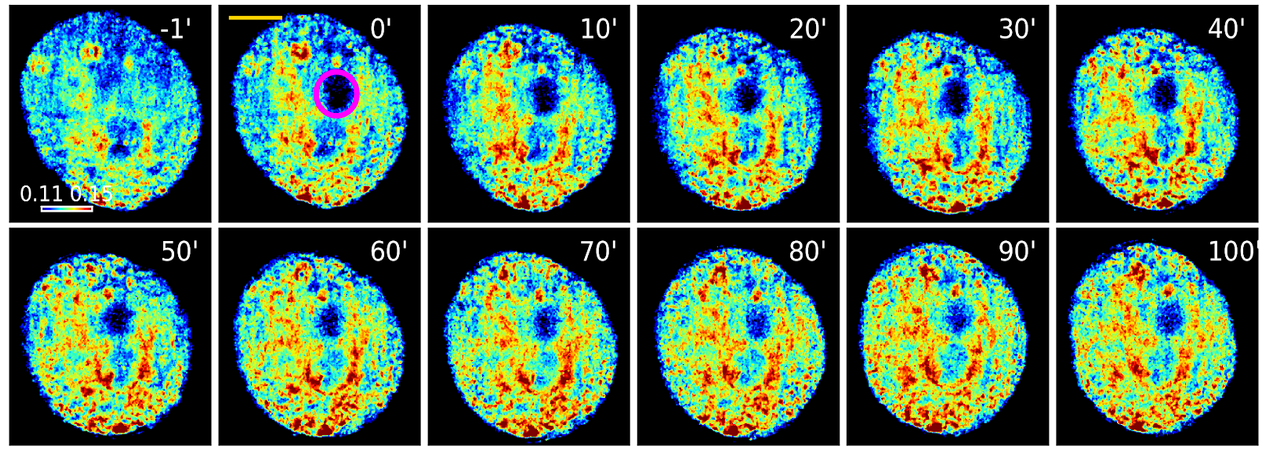
\includegraphics[clip,width=1\linewidth]{figures/live_an.png}\hspace*{\fill}}
    \caption{Dense nodes of chromatin are formed in microirradiated cells. H2B-EGFP anisotropy time series for a representative irradiated cell before and after irradiation, imaged every 5 min for over 2 h. The color map is scaled from 0.11 to 0.15. Scale bar corresponds to 5$\mu$m. Magenta circles indicate the sites of microirradiation.}
    {\label{fig:live_an}}
\end{figure}

\begin{figure}[H]
    {\hfill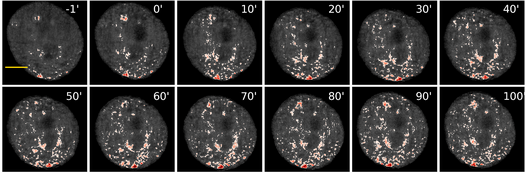
\includegraphics[clip, width=1\linewidth]{figures/thresholded.png}\hspace*{\fill}}
    \caption{A gray anisotropy map is plotted with color for anisotropy values greater than a threshold (mean + 2*standard deviation) calculated with respect to the -1' timepoint. The fraction of pixels above this constant threshold calculated for the -1' timepoint visibly grows with time indicating local compaction. Scale bar corresponds to 5$\mu$m.}
    {\label{fig:thresholded}}
\end{figure}

\begin{figure}[H]
    {\hfill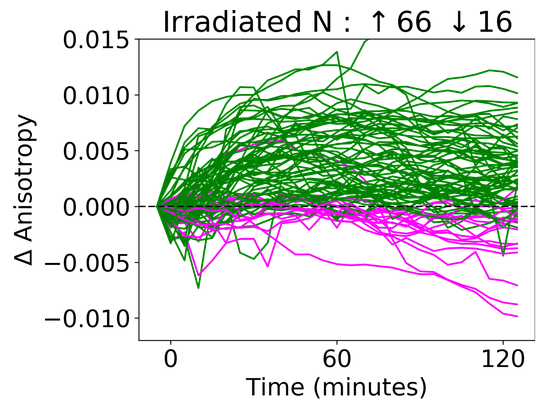
\includegraphics[clip, width=0.8\linewidth]{figures/closely.png}\hspace*{\fill}}
    \caption{Pooled single cell traces for irradiated cells done on three different days. 66 show a positive (green) trend and 16 a negative (magenta) trend.}
    {\label{fig:closely}}
\end{figure}


\paragraph*{} We microirradiated live cells and imaged them over 2 hours, every 5 minutes and computed their anisotropy maps (Fig. \ref{fig:live_an}). Since the 405nm laser bleaches EGFP locally, we could not obtain anisotropy information from the site of damage, but the anisotropy map of rest of the chromatin was unaffected. We quantified the change in anisotropy over time with $\Delta$Anisotropy, and found that as opposed to control (\(N=13\)), $\Delta$Anisotropy for irradiated cells (\(N=27\)) increased over time (Fig. \ref{fig:timetrace}). This indicated that there is increased compaction in the undamaged regions of chromatin in response to a local microirradiation. We fixed the cells after the course of imaging, and stained for common markers of DNA damage responses, and found that the phosphorylated form of DNA master kinase, ATM, forms nodes throughput the nucleus in a fraction of damaged cells (Fig. \ref{fig:patm}). These nodes are found in low anisotropy regions, indicating that these might be sites of damage repair. However, we were limited in observing the dynamics of repair factors, since fixing the cells destroys biological dynamics. In order to overcome this limitation, we utilized the chromobody technology (ChromoTek), and independently co-transfected H2B-EGFP expressing cells with chromobodies tagged with TagRFP against early and later markers of DDR, namely PARP1 and PCNA. Using this, we aimed to observe the dynamics of damage response in live cells, combined with chromatin compaction states as revealed by live anisotropy imaging.

\begin{figure}[H]
    {\hfill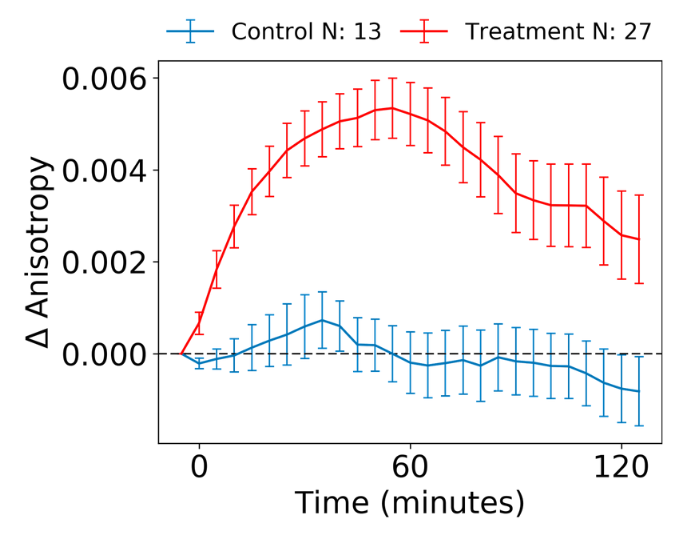
\includegraphics[clip, width=0.5\linewidth]{figures/timetrace.png}\hspace*{\fill}}
    \caption{$\Delta$Anisotropy is calculated by subtracting the mean anisotropy of any time point, with the mean anisotropy of the first time point for that cell. A positive $\Delta$Anisotropy corresponds to compaction, whereas a negative $\Delta$Anisotropy corresponds to decompaction.}
    {\label{fig:timetrace}}
\end{figure}


\begin{figure}[!htp]
    {\hfill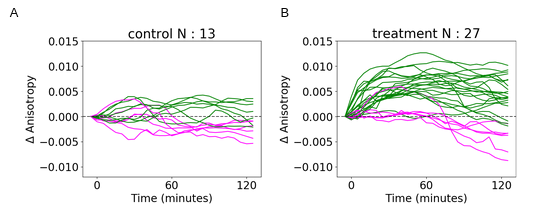
\includegraphics[clip, width=1\linewidth]{figures/hetero.png}\hspace*{\fill}}
    \caption{Compaction of undamaged chromatin in response to local damage.Individual $\Delta$anisotropy time traces of A. control (13 cells) and B. irradiated cells (27 cells). Cells with an overall positive trend are color-coded green, while those with a negative trend color-coded magenta. }
    {\label{fig:hetero}}
\end{figure}

\begin{figure}[!htp]
    {\hfill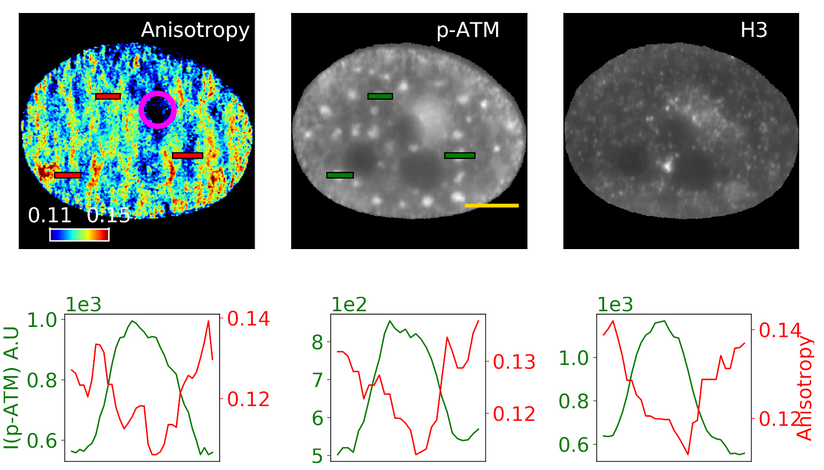
\includegraphics[clip, width=1\linewidth]{figures/patm.png}\hspace*{\fill}}
    \caption{Microirradiated cells are fixed after live imaging, and stained for damage markers. Phosphorylated-ATM is seen at sites of low anisotropy regions, and Histone H3 is accumulated at the site of damage. The purple circle is the site of microirradiation.}
    {\label{fig:patm}}
\end{figure}

\paragraph*{} PARP1 is a well characterized member of the poly (ADP ribose) polymerase (PARP) family of proteins, which are known to be transiently enhanced at sites of damage post microirradiation \cite{chou2010chromatin, qi2019multiple}. PARP1 is activated in the presence of broken DNA, which leads to the formation of poly (ADP ribose) (PAR), upon which further downstream repair factors are recruited. PCNA (proliferating cell nuclear antigen), a ring-shaped DNA replication cofactor, is a member of the family of DNA sliding clamps. It encircles DNA during replication, and enhances the processivity of DNA polymerase. PCNA is known to be associated with the final stages of DDR when new DNA has to be synthesized post excision of damaged DNA \cite{moldovan2007pcna}.

\begin{figure}[H]
    {\hfill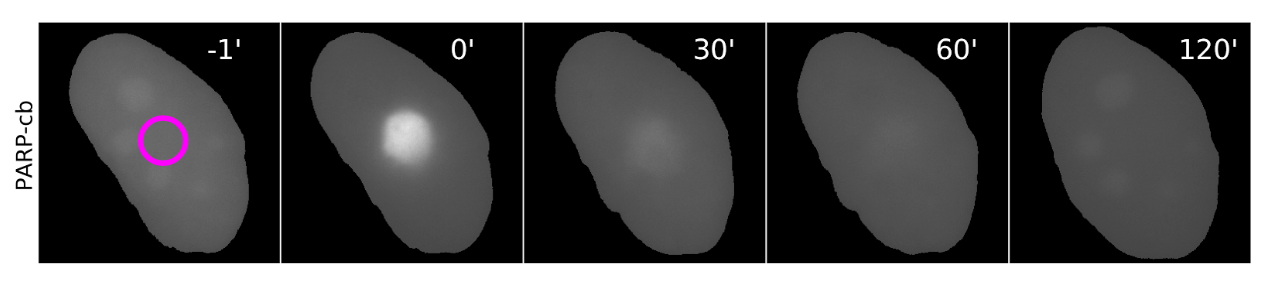
\includegraphics[clip, width=1\linewidth]{figures/parp.png}\hspace*{\fill}}
    \caption{Live cell dynamics of PARP-chrombody in irradiated cells, transiently transfected in HeLa H2B-EGFP cells. PARP1 showed immediate transient encrichment at the site of damage, and became homogenous quickly.}
    {\label{fig:parp}}
\end{figure}

\begin{figure}[H]
    {\hfill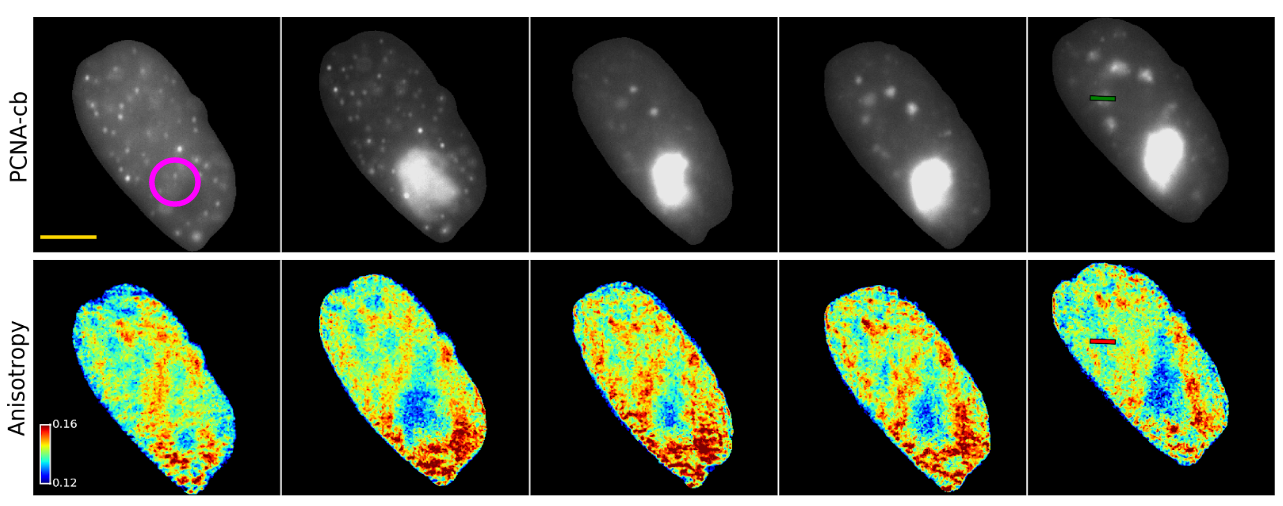
\includegraphics[clip, width=1\linewidth]{figures/pcna.png}\hspace*{\fill}}
    \caption{HeLa H2B-EGFP cells expressing PCNA chromobody along with its corresponding anisotropy maps, imaged at an  interval of 5 minutes post-irradiation. Scale bar corresponds to 5$\mu$m. Timestamps are same as (Fig. \ref{fig:parp})}
    {\label{fig:pcna}}
\end{figure}


\paragraph*{} We found that PARP1 was almost immediately recruited to site of damage upon microirradiation (Fig. \ref{fig:parp}), and diffused away from the site 15 minutes after damage. However, PCNA, which is a late stage repair protein, was also recruited immediately to the site of damage, and was found to be persistent at site of damage(Fig. \ref{fig:pcna}). We captured this behavior by quantifying the mean intensity of the chromobody at the site of damage, normalized to the mean intensity outside. (Fig. \ref{fig:retention})

\paragraph*{} While PCNA persists longer at the site of damage, within 20 minutes of irradiation, there are nodes of PCNA formed away form the site of damage. These nodes correspond to low-anisotropy regions, and incorporate EdU (ethynyl deoxyuridine), a thymidine analogue for labelling proliferating cells, suggesting that they are sites of damage repair.

\begin{figure}[H]
    {\hfill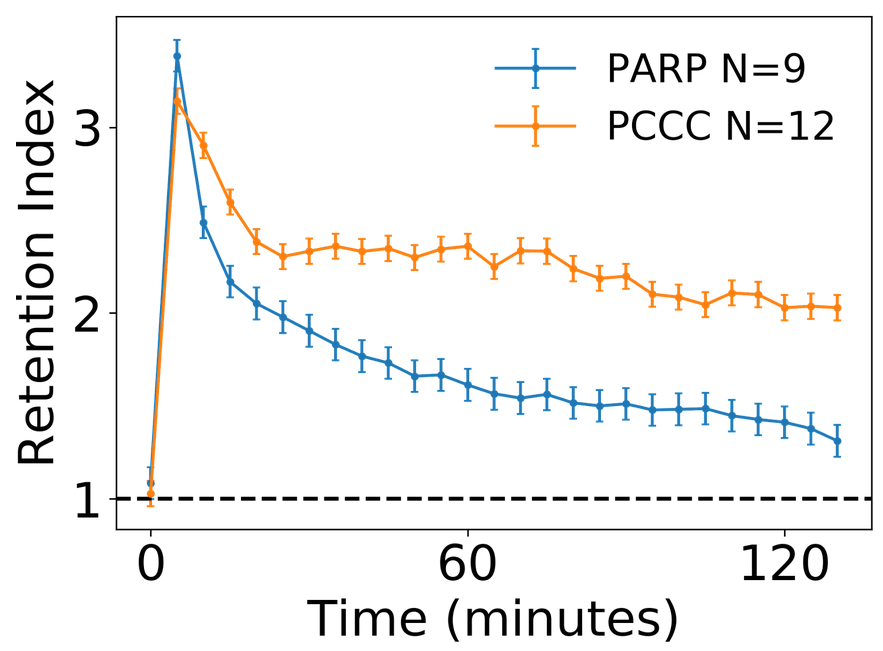
\includegraphics[clip, width=0.5\linewidth]{figures/retention.png}\hspace*{\fill}}
    \caption{PCNA persists at the site of damage longer than PARP. Retention index of any time point is defined as the ratio of intensity for a chromobody at the site of damage and outside the site of damage.}
    {\label{fig:retention}}
\end{figure}

\paragraph*{} We noticed that within 2 min after microirradiation, there is phosphorylation of Ser139 of the histone variant H2AX at the site of microirradiation, indicating DNA damage (Supplemental Figure 4). Although $\gamma$H2AX is a DNA damage marker, which is generally found as foci in regions of damaged chromatin, there is also a pan-nuclear spreading of $\gamma$H2AX in undamaged chromatin as early as 5 min after damage. In another study, interference with chromatin compaction at the damage site reduces the efficiency of damage repair. This suggested that condensation of chromatin is a necessary step in the activation of DDR (Burgess et al., 2014). However, ATM activation in mouse fibroblasts showed chromatin opening independent of DNA damage (Ji et al., 2017). During damage, ATM is thought to be activated not by direct binding to DNA strand breaks, but by changes in chromatin structure. Thus, forced compaction of chromatin promotes activation of ATR and ATM even where there are no strand breaks (Burgess et al., 2014), and conversely, activation of these kinases can change chromatin compaction (Becker et al., 2014). Thus, pan-nuclear induction of DDR (for which $\gamma$H2AX is a proxy) can drive compaction of undamaged chromatin, and the processes could feed back onto each other.

Such pan-nuclear induction of $\gamma$H2AX has been reported before when clustered DNA damage was induced by ionizing radiation, which is regulated by ATM and DNA-PK (Meyer et al., 2013). Other studies have discussed a ring of $\gamma$H2AX in the context of apoptosis (Solier and Pommier, 2014). It is possible that some of the cells we have irradiated will undergo apoptosis, and apoptotic response over and above the DNA damage response complicates the observed chromatin phenotypes. But apoptosis is accompanied by visible changes in the cell and nuclear morphology. However, our irradiated cells, under similar irradiation conditions, do not exhibit apoptotic morphology or fragmented chromatin, and many survive 48 h after irradiation. Furthermore, during the 2-h time course over which the cells were imaged, there was no significant induction of apoptotic or general cell death markers (Supplemental Figure 9). This indicates that the compaction we observe may have to do with the early processes of DDR rather than the long-term processes of cell death because of excessive DNA damage.

PCNA, surprisingly, is shown to be recruited immediately to the site of localized DSBs, independent of cell-cycle phase. As interestingly, at longer time-points it forms transient nodes of repair away from the site of damage in regions of more open chromatin (low anisotropy). These nodes actively incorporate EdU, indicating active repair and possibly a looping of DSBs from the primary laser-induced cluster to open regions of chromatin for the purposes of repair.

Our study establishes the possibility of using FAI to measure chromatin compaction changes in the context of DNA damage in living cells, followed by immunofluorescence for DDR and chromatin markers. While the response to DSBs is investigated here, following previous studies (Kruhlak et al., 2006; Burgess et al., 2014), in principle, the method is amenable to other forms of DNA damage as well, which we aim to investigate in the future.

\paragraph*{} In summary, we observed the dynamics of chromatin compaction state, and correlated it with markers of damage, such as phosphorylated ATM, which forms nodes at low anisotropy regions. We found that damage repair markers have different dynamics, as PARP1 has low retention in the site of damage, as opposed to PCNA, which persists for longer time period. We also observed that PCNA forms nodes of repair, away from the site of damage, which correspond to regions of low anisotropy and EdU incorporation.





 Next we wanted to combine the time course of anisotropy imaging with live-cell detection of other markers of the damage response. For this, we chose chromobody-mediated detection of early and late markers of DDR—PARP1 and PCNA. PARP1 is known to be transiently enhanced at sites of damage in response to irradiation-induced DSBs (Chou et al., 2010; Qi et al., 2019), while PCNA, being the DNA clamp, would be required for the processivity of the DNA polymerase in the final steps of repair (Moldovan et al., 2007). We independently transfected PARP1 and PCNA chromobodies tagged with TagRFP in HeLa cells stably expressing H2B-EGFP. Chromobodies (ChromoTek) are small intracellular antibodies tagged with fluorescent protein. Their major advantage is that they detect the endogenous proteins they are designed against without artifacts of overexpression of those proteins in transient transfections (Burgess et al., 2012; Panza et al., 2015). As expected, PARP1 was recruited to the site of damage almost immediately upon irradiation (Figure 3A). However, the PARP1 signal diffused away from the site by 15 min after damage, as expected (Haince et al., 2008; Mortusewicz et al., 2007). To our surprise, however, PCNA, which should be involved in the repair only at later stages, was also recruited immediately to the site of damage (Figure 3B). This was the case in G1 and G2 cells where the PCNA chromobody was homogenous in the nucleus, and even in S phase cells where the PCNA chromobody was punctated, as PCNA follows the replication fork (Supplemental Movies 1 and 2). The PCNA chromobody is primarily used for cell-cycle stage detection (Burgess et al., 2012). This implies that in response to clustered DSBs, even PCNA from replication forks is recruited to the site of damage. PCNA persisted at the site of damage for the duration of the time course, longer than PARP1 (Figure 3C). This local enrichment was quantified by plotting the mean intensity of the chromobody at the site of damage normalized to the mean intensity outside. (We found this to be a more robust metric for the enrichment, compared with just the normalized intensity at the site of damage, which decays due to photobleaching during the time course, in addition to actual dynamics. This metric is more robust because photobleaching operates both within and outside the site of damage.) But while PCNA persists longer, within 20 min, there are nodes of PCNA formed, away from the site of damage, which correspond to regions of lower anisotropy (Figure 3; Supplemental Figure 6). We asked whether these sites of PCNA enrichment and low anisotropy represent simply sites of repair factor storage or of active repair. We reasoned that if they are indeed sites of repair, even in the G1 or G2 phase, we may be able to see incorporation of a deoxynucleotide analog such as ethynyl deoxyuridine (EdU). HeLa cells transfected with the PCNA chromobody were subjected to laser-induced DSBs. G1 or G2 cells that have a homogenous distribution of the PCNA chromobody in the nucleus were chosen. We observed that at these sites of transient PCNA nodes, EdU is incorporated, which is an indication of new DNA being synthesized at these sites (Figure 3E; Supplemental Figure 7). We ruled out bleedthrough of PCNA signal in the EdU channel by imaging plates for cells with and without EdU treatment (Supplemental Figure 7). Thus, though the DSBs are induced locally, these nodes of PCNA incorporating EdU further away may indicate a looping out of individual DSBs from the site of primary damage.


 In the context of DDR, our fluorescence anisotropy imaging studies suggest that the undamaged chromatin is globally compacted in response to localized DSB damage. In regions away from the site of damage, we observe chromatin nodes forming, as well as transient accumulation of phospho-ATM and PCNA in specific sites that correspond to more loosely packed regions of chromatin. These low-anisotropy regions with accumulated repair proteins could be regions of repair or of factors poised for repair. In future studies, we aim to investigate the possibility of blocking damage response in cells using small molecule inhibitors for DDR master kinases and what effects it has on the chromatin response upon damage. A limitation of this study is that we follow the response of undamaged chromatin because of local clustered DSBs, but anisotropy information is lost at the site of damage because of photobleaching. This could potentially be circumvented by using a histone H2B tagged with photoactivable GFP (H2B-PA-GFP). Condensation of the damaged chromatin could indeed be observed in such an experiment (Supplemental Figure 8).
